\documentclass{article}
\usepackage[utf8]{inputenc}
\usepackage{cmap}
\usepackage[T2A]{fontenc}
\usepackage[english,russian]{babel}
\usepackage{amsmath,amsfonts,amssymb,amsthm,mathtools}
\title{Диффузия}
\author{Шмаков Владимир Евгеньевич}
\date{МФТИ, апрель 2022}
\title{Определение $\frac{C_p}{C_v}$ по скорости звука}

\begin{document}

\maketitle

\newpage

\section{Цель работы}
\begin{enumerate}
    \item Измерить резонансные частоты колебаний в трубе, заполненной газом
    \item По полученным данным оценить сокрость звука в газе
    \item Убедиться в зависимости скорости звука от температуры окружающей среды
    \item Вычислить показатель адиабаты $\gamma = C_{p}/C_{v}$
\end{enumerate}
\section{Оборудование}
\begin{itemize}
    \item Генератор сигналов
    \item Шикорокополосный динамик и микрофон
    \item Осциллограф
    \item Термостат
    \item Теплоизолированная труба
\end{itemize}
\section{Эксперементальная установка и некоторые теоретические данные}
\subsection{Условие возникновения резонанса}
Рассмотрим колебательный процесс проходящий по гармоническому закону:
\begin{equation}\label{HarmonicOscillationProcess}
    U(x,y,z,t) = \Psi(x,y,x) \cdot \cos{\omega t}
\end{equation}
Где $U(x,y,z,t)$ - Возмущение в данной точке в момент времени $t$
Воспользуемся волновым уравнением:
\begin{equation}\label{waveEquation}
   \frac{ \partial^2 U}{\partial x^2} + \frac{ \partial^2 U}{\partial y^2} + \frac{ \partial^2 U}{\partial z^2} = \frac{1}{C_{\text{звука}}} \cdot \frac{\partial^2 U}{\partial t^2}
\end{equation}
Продифференцировав выржение \eqref{HarmonicOscillationProcess} дважды по времени, и выразив из \eqref{waveEquation} второй дифференциал возмущения по времени получим волновое уравнение для синусоидальных колебаний:
\begin{equation}\label{mainHarmEq}
    \Delta \Psi + k^2 \Psi = 0
\end{equation}
Где $\Delta \Psi$ - оператор лапласа содержащий вторые частные производные (аналогично левой части уравнения \eqref{waveEquation})
\newpage
Для возникновения стоячей волны необходимо избежать разности фаз между излучаемой и отраженной волнами:
\begin{center}
\includegraphics[scale = 0.5]{StaticWawes.jpg}
\end{center}
Другими словами, на концах трубы должен фозникать <<узел>>:
\begin{equation}\label{staticWaveCondition}
    \frac{\partial \Psi}{\partial x} = 0  \text{ в точках }
    x = 0, x = L
\end{equation}
Решаем уравнение \eqref{mainHarmEq}, используя условие \eqref{staticWaveCondition}. В результате некоторых промежуточных преобразований получаем формулу для вычисления <<собственных>> частот трубы, как колебательной системы:
\begin{equation}\label{resonance}
    f_{n} = \frac{n C_{\text{звука}}}{2L}
\end{equation}
\subsection{Скорость звука в газе}

Скорость продольной волны определяется соотношением $C_{\text{звука}}^2 = d P/ d \rho$. 

Существовало две теории распространения звуковых волн. Верной оказалась теория Лапласа о том, что этот процесс адиабатический. 
Тогда:
\begin{equation}\label{speedOfSound}
C_{\text{звука}}^2 = \frac{\gamma R T}{\mu}
\end{equation}
где $\gamma$ - показатель адиабаты ($\gamma = C_{p}/C_{v}$)
\subsection{Методика измерений}
\begin{center}
    \includegraphics[scale = 0.7]{schematic.png}
\end{center}

Приблизительно оценим диапазон частоты первой гармоники. Настраивая частоту на генераторе, добиваемся максимальной амплитуды. Таким образом, делая пять измерений получаем первые пять резонансных гармоник.

Для оценки зависимости скорости звука от темепратуры, повторим измерения при разных значениях температуры на термостате.
\section{Результаты измерений}

В результате 5 экспериментов при температурах $22.4^\circ C$, $28.3^\circ C$,
$33.0^\circ C$, $38.1^\circ C$, $43.1^\circ C$, $48.1^\circ C$ получены следующие резонансные частоты:
\begin{center}
    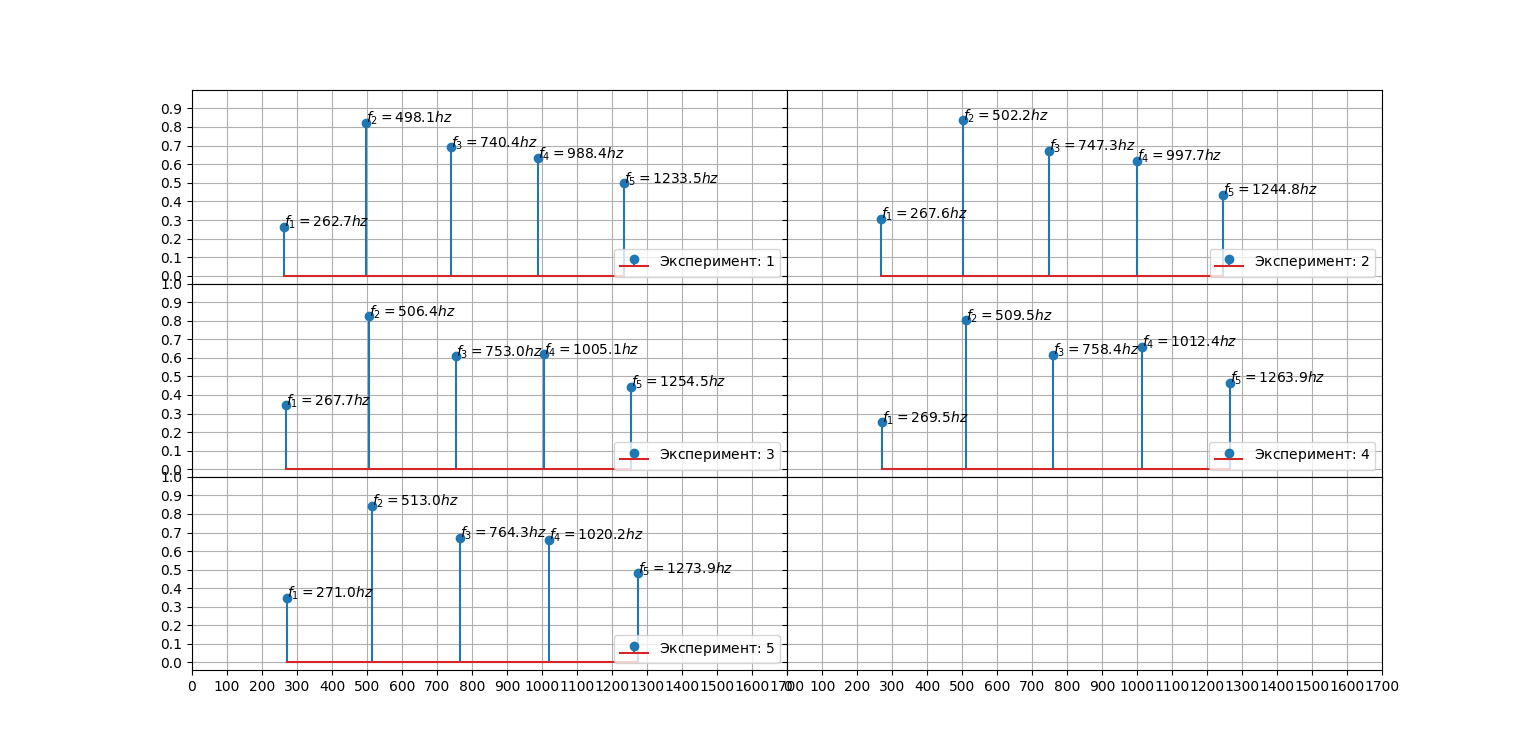
\includegraphics[scale = 0.3]{expResults.png}
\end{center}
\section{Обработка результатов эксперимента}

Согласно формуле 
\begin{equation}
    f_{k+1} = \frac{C_{\text{звука}}}{\lambda_{k+1}}
\end{equation}
коэффициент наклона прямой зависимости $f_{n}-f_{0}$ от $n$ есть $C_{\text{звука}}/2L$.

Построим графики зависимости $f_{n}-f_{0}$ от $n$(см. приложение) и методом наименьших квадратов вычислим коэффициенты наклона прямых. Умножив полученное значение $\alpha$ на $2L$, получим скорость звука при данной температуре.

Из фомулы \eqref{speedOfSound} выразим показатель адиабаты:
\begin{equation}
    \gamma = \frac{\mu}{R T} \cdot C_{\text{звука}}^2
\end{equation}

Получены следующие результаты:
\newpage
\begin{table}[h]
\centering
\begin{tabular}{ l c c r }
$ \text{Эксепримент 1} $ & $T_{1} = 295.4 \pm 0.2 K$ & $C_{s1} = 340 \pm 7 \frac{m}{s}$ & $\frac{C_{p}}{C_{v}}_{1} = 1.40 \pm 0.05 $\\
$ \text{Эксепримент 2} $ & $T_{2} = 301.0 \pm 0.2 K$ & $C_{s2} = 343 \pm 7 \frac{m}{s}$ & $\frac{C_{p}}{C_{v}}_{2} = 1.40 \pm 0.06 $\\
$  \text{Эксепримент 3}$ & $T_{3} = 306.0 \pm 0.2 K$ & $C_{s3} = 336 \pm 7 \frac{m}{s}$ & $\frac{C_{p}}{C_{v}}_{3} = 1.40 \pm 0.06 $\\
$ \text{Эксепримент 4} $ & $T_{4} = 311.0 \pm 0.2 K$ & $C_{s4} = 349 \pm 7 \frac{m}{s}$ & $\frac{C_{p}}{C_{v}}_{4} = 1.40 \pm 0.06 $\\
$ \text{Эксепримент 5} $ & $T_{5} = 316.0 \pm 0.2 K$ & $C_{s5} = 352 \pm 7 \frac{m}{s}$ & $\frac{C_{p}}{C_{v}}_{5} = 1.40 \pm 0.06 $\\
\end{tabular}
\end{table}
\section{Вывод}
С точностью $\approx 2\%$ удалось получить скорость звука при различных температурах. 
Сравним значение с табличным. Согласно источнику <<сетвая метерология>>\footnote{https://www.meteorologiaenred.com/ru/} скорость звука при комнатной температуре составляет $343 m/s$, что в пределах погрешности совпадает со значением, полученным в первом эксперименте.

Рассматривая воздух как двухатомный идеальный газ:
\begin{equation*}
    \gamma = \frac{C_p}{C_v} = \frac{7}{2} \cdot \frac{2}{5} = 1.4
\end{equation*}
Именно такое значение было получено в проведенных экспериментах.

Как видно из формулы \eqref{speedOfSound}, скорость звука увеличивается с ростом температуры, что потверждают результаты опыта. И зависимость скорости звука от температуры линейная. Однако диапазон температур оказался малым для оценки типа зависимости. Используя различную аппроксимацию, и учитывая все точки попавшие в <<крест>> погрешностей, можем получать различные виды зависимостей:
\begin{center}
    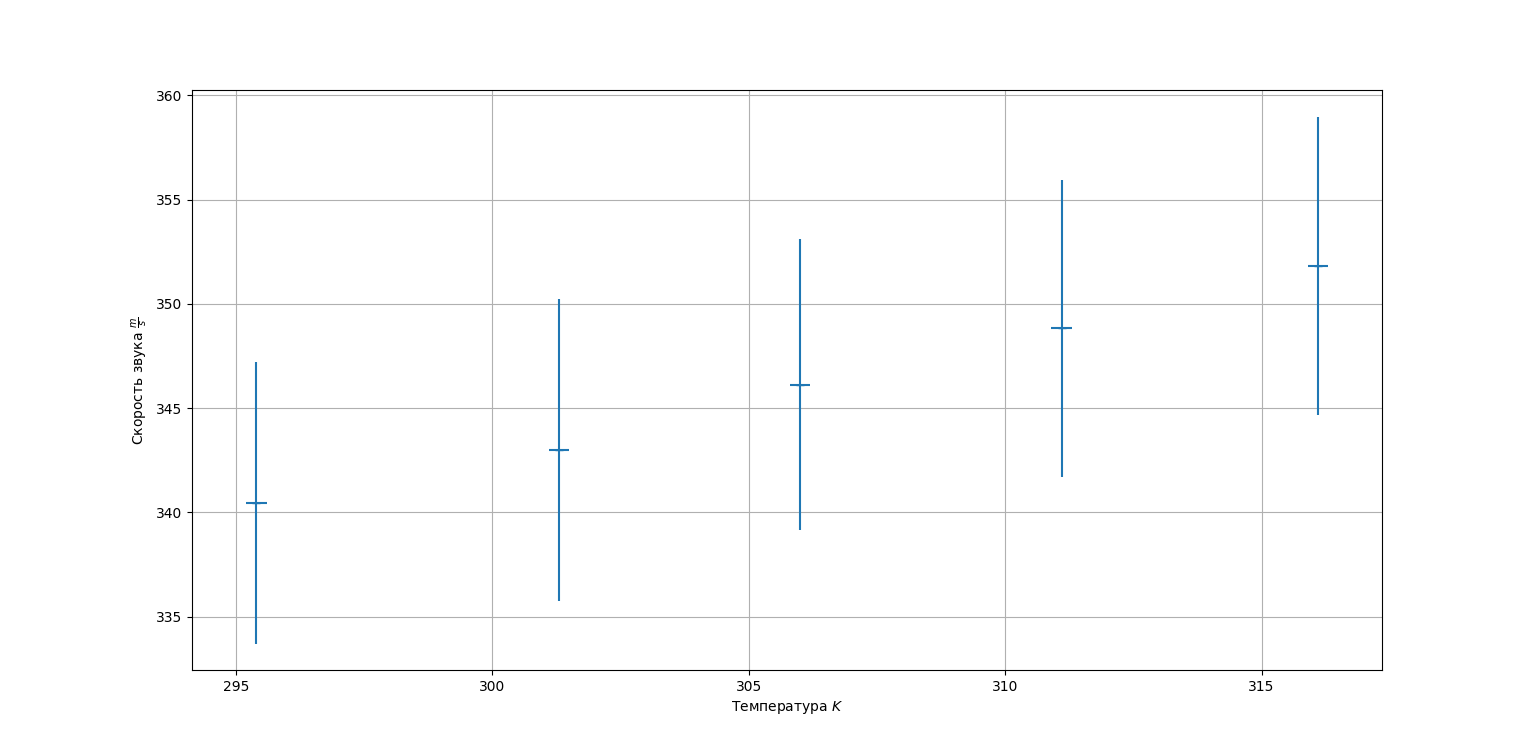
\includegraphics[scale = 0.25]{sppedByT.png}
\end{center}

Подробно ознакомиться с рассчетами можно по сслыке\footnote{https://github.com/ShmakovVladimir/Labs}
\section{Приложение}

\end{document}
